% Chapter 4

\chapter{Results}

\label{Chapter4}

We begin our discussion of the results with preliminary analysis of the data that helped shape the experimental design. Here we seek to understand what are some of the overarching patterns in music listening habits and how these look at an individual level.

After this we present a summary of our results followed by a discussion of the performance of each individual method.

\section{Preliminary analysis}

\subsection{Daily play patterns}

By grouping track plays into 30 min intervals and aggregating by periods within a day, we see a clear daily pattern with music listening hitting a peak at around 5pm and a trough at around 6am.

\begin{figure}[h!]
	\centering
	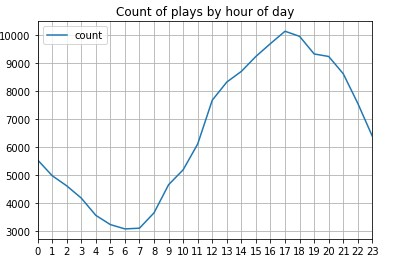
\includegraphics[width=7cm, keepaspectratio,]{fig004.jpg}
	\caption{5-5.30pm is peak listening time}
	\label{3a}
\end{figure} 

Zooming out to view the pattern across an entire week in figure \ref{3b}, we see that the daily pattern occurs across every day of the week with weekends having a lower total number of plays.

\begin{figure}[h!]
	\centering
	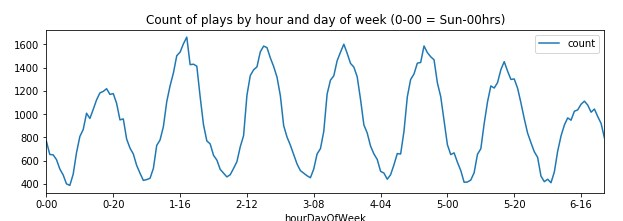
\includegraphics[width=7cm, keepaspectratio,]{fig005.jpg}
	\caption{Most popular times to listen to music across all users}
	\label{3b}
\end{figure} 

At a high level therefore one can get good accuracy by simply anticipating music demand to peak at 5pm. However if we select two users at random, we see (see fig. \ref{3c}) that these daily patters are not as strongly discernable. This demonstrates why models modeling the high levels patterns is not enough for individual user prediction. 

\begin{figure}[h!]
	\centering
	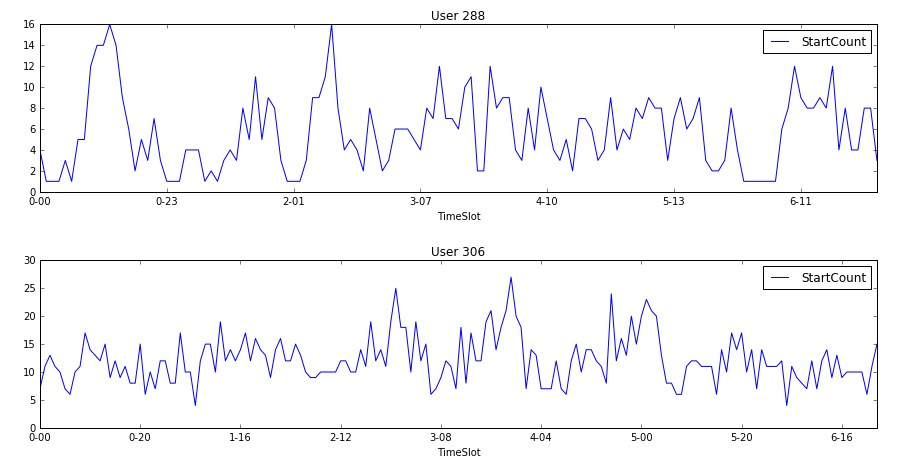
\includegraphics[width=7cm, keepaspectratio,]{fig006.jpg}
	\caption{Most popular times to listen to music by individual user}
	\label{3c}
\end{figure} 

\subsection{Inter-event times}

The dataset contains a timestamp associated with each user. This does not necessarily mean the user played a song in its entirety. Analysis shows plenty of cases where the interval time between tracks was a few seconds suggesting the user skipped tracks. 

Figure \ref{3d} shows a frequency plot of intervals. Intervals beyond 30 minutes continue the exponential decrease and are not shown. We see that while the mode is on par with a typical song length, there is a significant number of plays that lasted under 5 minutes. 

\subsection{Time-series analysis}

Here we examine our data once it has been transformed in a binary sequence of events (1) and non-events(0). We seek to understand better how an optimizer may perform based on traits of the data.

We begin with assessing how well our baseline model may perform based on assuming $t = t-1$. Fig \ref{fig12} shows that the 76\% of Plays, also had a play in t-1. However simply using this as a rule would also capture 2.2\% of non-plays.

\begin{figure}[h!]
	\centering
	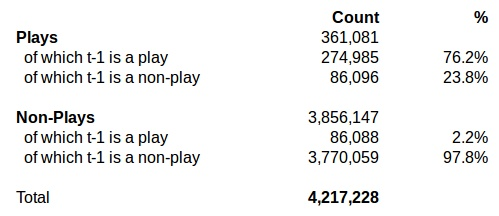
\includegraphics[width=7cm, keepaspectratio,]{fig012.jpg}
	\caption{}
	\label{fig12}
\end{figure} 

Furthermore the 23.8\% of Plays that did not have a Play in the prior period are harder to predict yet of more interest as they representthe beginning of the listneing period and therefore more useful to a music recommender system. 

Given the daily patterns we have seen, it might be reasonable to assume that looking at the same period 24 hours prior may be a good indicator of whether t is a play event. However as we see from fig. \ref{fig12b} this is not a reliable indicator either.

\begin{figure}[h!]
	\centering
	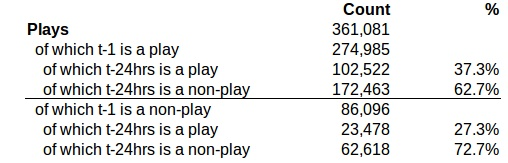
\includegraphics[width=7cm, keepaspectratio,]{fig012b.jpg}
	\caption{}
	\label{fig12b}
\end{figure} 

What both of these results tell us is that fairly high precision score of around 76\% ought ot be possible purely based on t-1 but going above this while having a good precision score on the non-play events will be harder.

Finally it was found that of rows where all timelags had a non-play event, 0.62\% of rows had a play event. As this was a low number it was deemed safe to remove all such rows from the dataset in order to improve the speed and quality of analysis. 

\subsection{Outliers}

The data was checked for any unusual outliers that may impinge upon the goal of developing a model to predict user behaviour. An analysis of plays by user reveals a high amount of variance between users on how many tracks are played. 

\begin{figure}[h!]
	\centering
	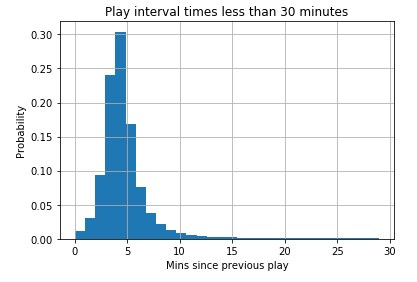
\includegraphics[width=7cm, keepaspectratio,]{fig003.jpg}
	\caption{}
	\label{3d}
\end{figure} 

For our purposes these are include as evidence that the user was interested in playing music at time $t$.

We can also assume that the song plays are not independent of one another, in that the probability of a play event at time t+1 is significantly higher if there was an event at time t. 


\subsection{Outliers}

The data was checked for any unusual outliers that may impinge upon the goal of developing a model to predict user behaviour. An analysis of plays by user reveals a high amount of variance between users on how many tracks are played. 

\begin{figure}[h!]
	\centering
	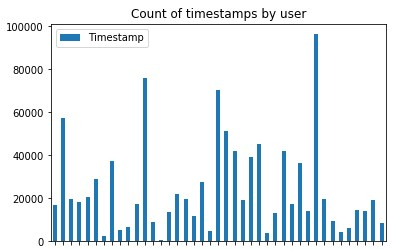
\includegraphics[width=7cm, keepaspectratio,]{fig002.jpg}
	\caption{Total play count by user}
	\label{fig2}
\end{figure} 


\newpage

Further analysis showed one user in particular with very high amount of plays, with very low durations, suggesting it was likely to have been generated by a bot, possibly a LastFM test. This was excluded from the dataset.

\section{Main results} % Methodology

We will now present the results of the experiments conducted. We start with a summary of the results obtained through 5-fold cross validation then discuss our results in more depth.

Fig. \ref{fig13a} shows the overall results from 5-fold cross validation. From this it would appear that almost all models outperformed the baseline model. However these results disguise the true picture. The precision and recall are the average across both plays and non-plays.  We can instead look at 'first play' events only (fig. \ref{fig13b}) by defining 'first play' as any plays where there were no plays in the previous 4 perids (i.e.2 hours). Here we see a more mixed pattern with SVM models scoring an average 81\% on precision, logistic regression an average of 68\% on recall, and the Baseline and Bayesian models performing significantly worse. 

\begin{figure}[h!]
	\centering
	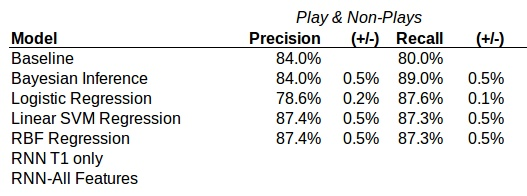
\includegraphics[width=8cm, keepaspectratio,]{fig013a.jpg}
	\caption{}
	\label{fig13a}
\end{figure} 

 
 
\begin{figure}[h!]
	\centering
	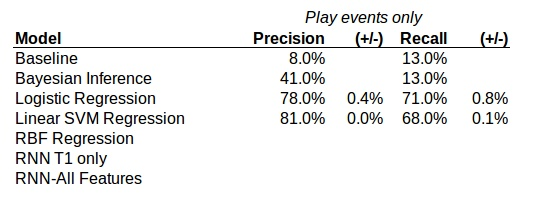
\includegraphics[width=8cm, keepaspectratio,]{fig013b.jpg}
	\caption{}
	\label{fig13b}
\end{figure}  



\section{RNN-LSTM}

The RNN model required a lot more effort to set up and get meaningful results from. While some of this was down to how Tensorflow operates, some of it is also a feature of deep leanting itself. In the quest to find a model that worked the following tweak were made to the starting model.

\textit{Computational efficiency}

RNN's require the construction of a 3-dimensional tensor in which the second dimension is unstacked to create a list of timesteps. Using pre-allocated arrays than appending to arrays was found to provide a significan speed boost in shaping the data in theis way.

\textit{Data Sampling}

It is well known that deep learning requires a large amount of data from which to learn from. In order to provide it within enough varied data the following hierarchy of iteration was set up up:

\begin{enumerate}
	\item Sampling iteration (s)
	\item Period iteration (p)
	\item Batch iteration (n) and Batch size (z)
\end{enumerate}

The highest level of iteration was a sampling iteration, S. Each sampling iteration selects a user at random.  For each random user p random periods were selected. For each period selected z preceding periods were selected to form a single batch of training data. This model was then fed this batch n times.

Further traning parameters was the number of hidden notes, h, in the RNN; and the number of timesteps, selected for each row of the batch.

It was oberved that a variery of training data, particularly from different users, was more beneficial than  high amount of iteraions or a deeper network.

Figure <TBC> shows the performance across different parameter settings, with the best result across all models shown in <TBC>

\begin{figure}[h!]
	\centering
	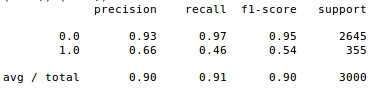
\includegraphics[width=7cm, keepaspectratio,]{fig011.jpg}
	\caption{}
	\label{fig:fig11}
\end{figure} 


\section{Overall results summary}

The best scores per model are shown in figure \ref{fig9}.
Looking at the F1-score we see that the Logistic regression model performs the best. It was also found to be consistent across different runs of the model.


\begin{figure}[h!]
	\centering
	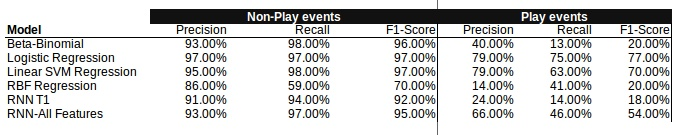
\includegraphics[width=12cm, keepaspectratio,]{fig009_Results.jpg}
	\caption{Summary of best scores}
	\label{fig9}
\end{figure} 

TO BE COMPLETED

\section{Adaptability to new users}

One of our areas of interest was how accurate such models are when it comes to learning the patterns of new users. Tie figures below show how the accuracy improved over time for each of the 10 test users. The periods indicate half-hourly intervals with 2-3,000 periods (1.5-2 months) appearing to be the time it takses to learn the habits of a typical user. 
\begin{figure}[h!]
	\centering
	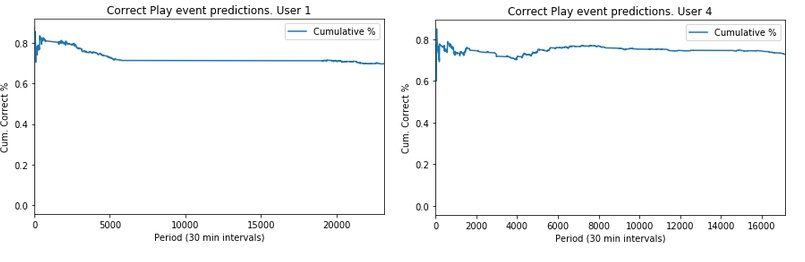
\includegraphics[width=7cm, keepaspectratio,]{fig008a.jpg}
	\caption{}
	\label{fig:fig8a}
\end{figure} 

\begin{figure}[h!]
	\centering
	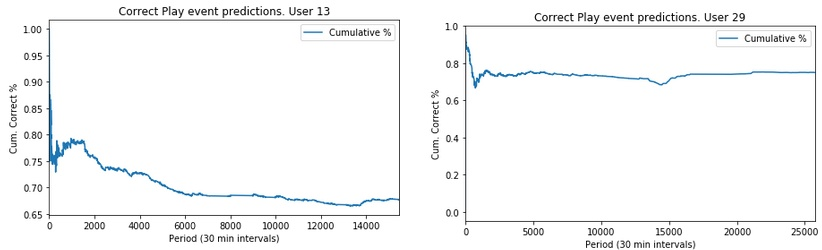
\includegraphics[width=7cm, keepaspectratio,]{fig008b.jpg}
	\caption{}
	\label{fig:fig8b}
\end{figure} 

\begin{figure}[h!]
	\centering
	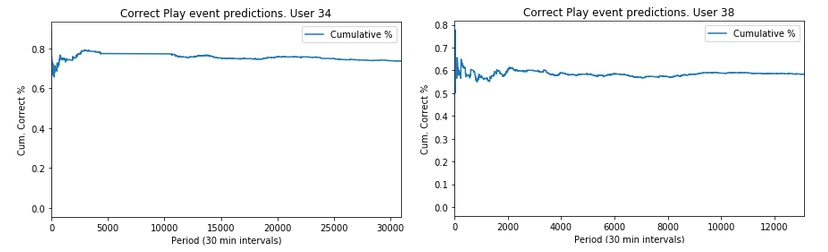
\includegraphics[width=7cm, keepaspectratio,]{fig008c.jpg}
	\caption{}
	\label{fig:fig8c}
\end{figure} 

\begin{figure}[h!]
	\centering
	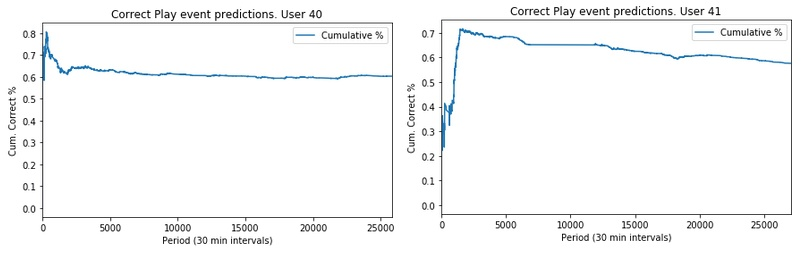
\includegraphics[width=7cm, keepaspectratio,]{fig008d.jpg}
	\caption{}
	\label{fig:fig8d}
\end{figure} 

\begin{figure}[h!]
	\centering
	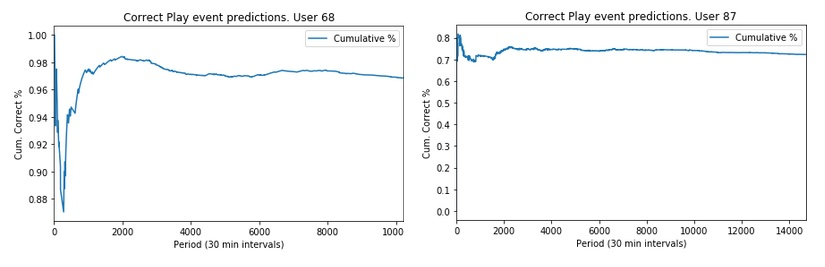
\includegraphics[width=7cm, keepaspectratio,]{fig008e.jpg}
	\caption{}
	\label{fig:fig8e}
\end{figure} 


From these charts it appears that two months worth of data is required to for the model to rget trained up on a new user.
